% Created 2021-01-20 Wed 07:39
% Intended LaTeX compiler: pdflatex
\documentclass[presentation]{beamer}
\usepackage[utf8]{inputenc}
\usepackage[T1]{fontenc}
\usepackage{graphicx}
\usepackage{grffile}
\usepackage{longtable}
\usepackage{wrapfig}
\usepackage{rotating}
\usepackage[normalem]{ulem}
\usepackage{amsmath}
\usepackage{textcomp}
\usepackage{amssymb}
\usepackage{capt-of}
\usepackage{hyperref}
\usetheme{Luebeck}
\author{Abraham Raji}
\date{January 23, 2020}
\title{The Linux Circle Designer}
\subtitle{The story of how my love for free software turned me into a designer}}
\titlegraphic{
\includegraphics[height=.1\textheight]{./logo.png}}
\hypersetup{
 pdfauthor={Abraham Raji},
 pdftitle={The Linux Circle Designer},
 pdfkeywords={foss design},
 pdfsubject={State of FOSS Design},
 pdfcreator={Emacs 27.1 (Org mode 9.5)}, 
 pdflang={English}}
\begin{document}

\maketitle

\section*{My Story}
\label{sec:orgfe801a6}
\begin{frame}[label={sec:orgbc8cf46},fragile]{About the 2018 Me}
 \begin{columns}
\begin{column}{0.5\columnwidth}
\begin{itemize}
\item Abraham Raji a.k.a \texttt{avronr}
\item Loves Programming.
\item Free/Libre Software Enthusiast.
\item Ran a FOSS club at my college.
\end{itemize}
\end{column}
\begin{column}{0.5\columnwidth}
\begin{figure}[htbp]
\centering
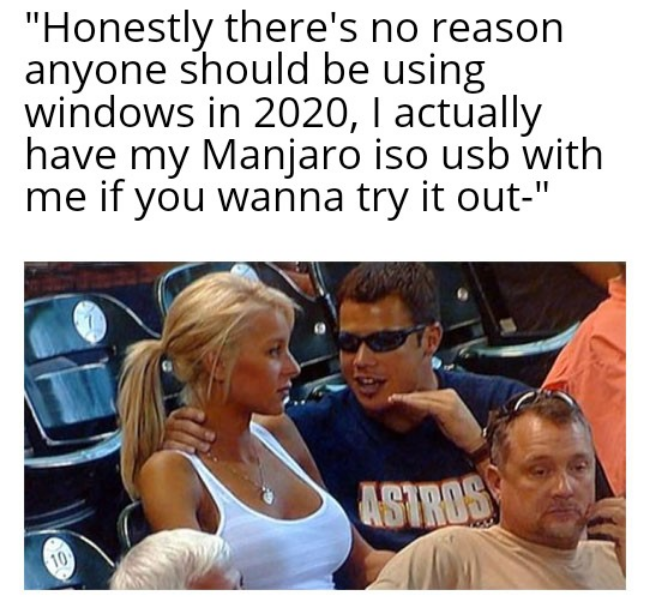
\includegraphics[height=40mm]{././meold.png}
\caption{A picture of me 2018}
\end{figure}
\end{column}
\end{columns}
\end{frame}
\begin{frame}[label={sec:org0d6dc39}]{I started designing.}
\begin{columns}
\begin{column}{0.7\columnwidth}
\begin{itemize}
\item College events by the FOSS club required posters.
\item Most Designers used the Adobe Suite.
\item I didn't wanna let Stallman down
\item Finding Raghavendra Kamath.
\item So I decided to give it a try myself.
\end{itemize}
\end{column}
\end{columns}
\end{frame}
\section*{Stuff I've done}
\label{sec:org7df3c4e}
\begin{frame}[label={sec:orgaf4c7a7}]{Now I design}
\begin{columns}
\begin{column}{0.25\columnwidth}
\begin{figure}[htbp]
\centering

\includegraphics[width=.9\linewidth]{././onam4.png}
\caption{Onam, SDS (2020)}
\end{figure}
\end{column}
\begin{column}{0.25\columnwidth}
\begin{figure}[htbp]
\centering

\includegraphics[width=.9\linewidth]{././theyyam.png}
\caption{Announcement, DebConf (2020)}
\end{figure}
\end{column}
\begin{column}{0.25\columnwidth}
\begin{figure}[htbp]
\centering
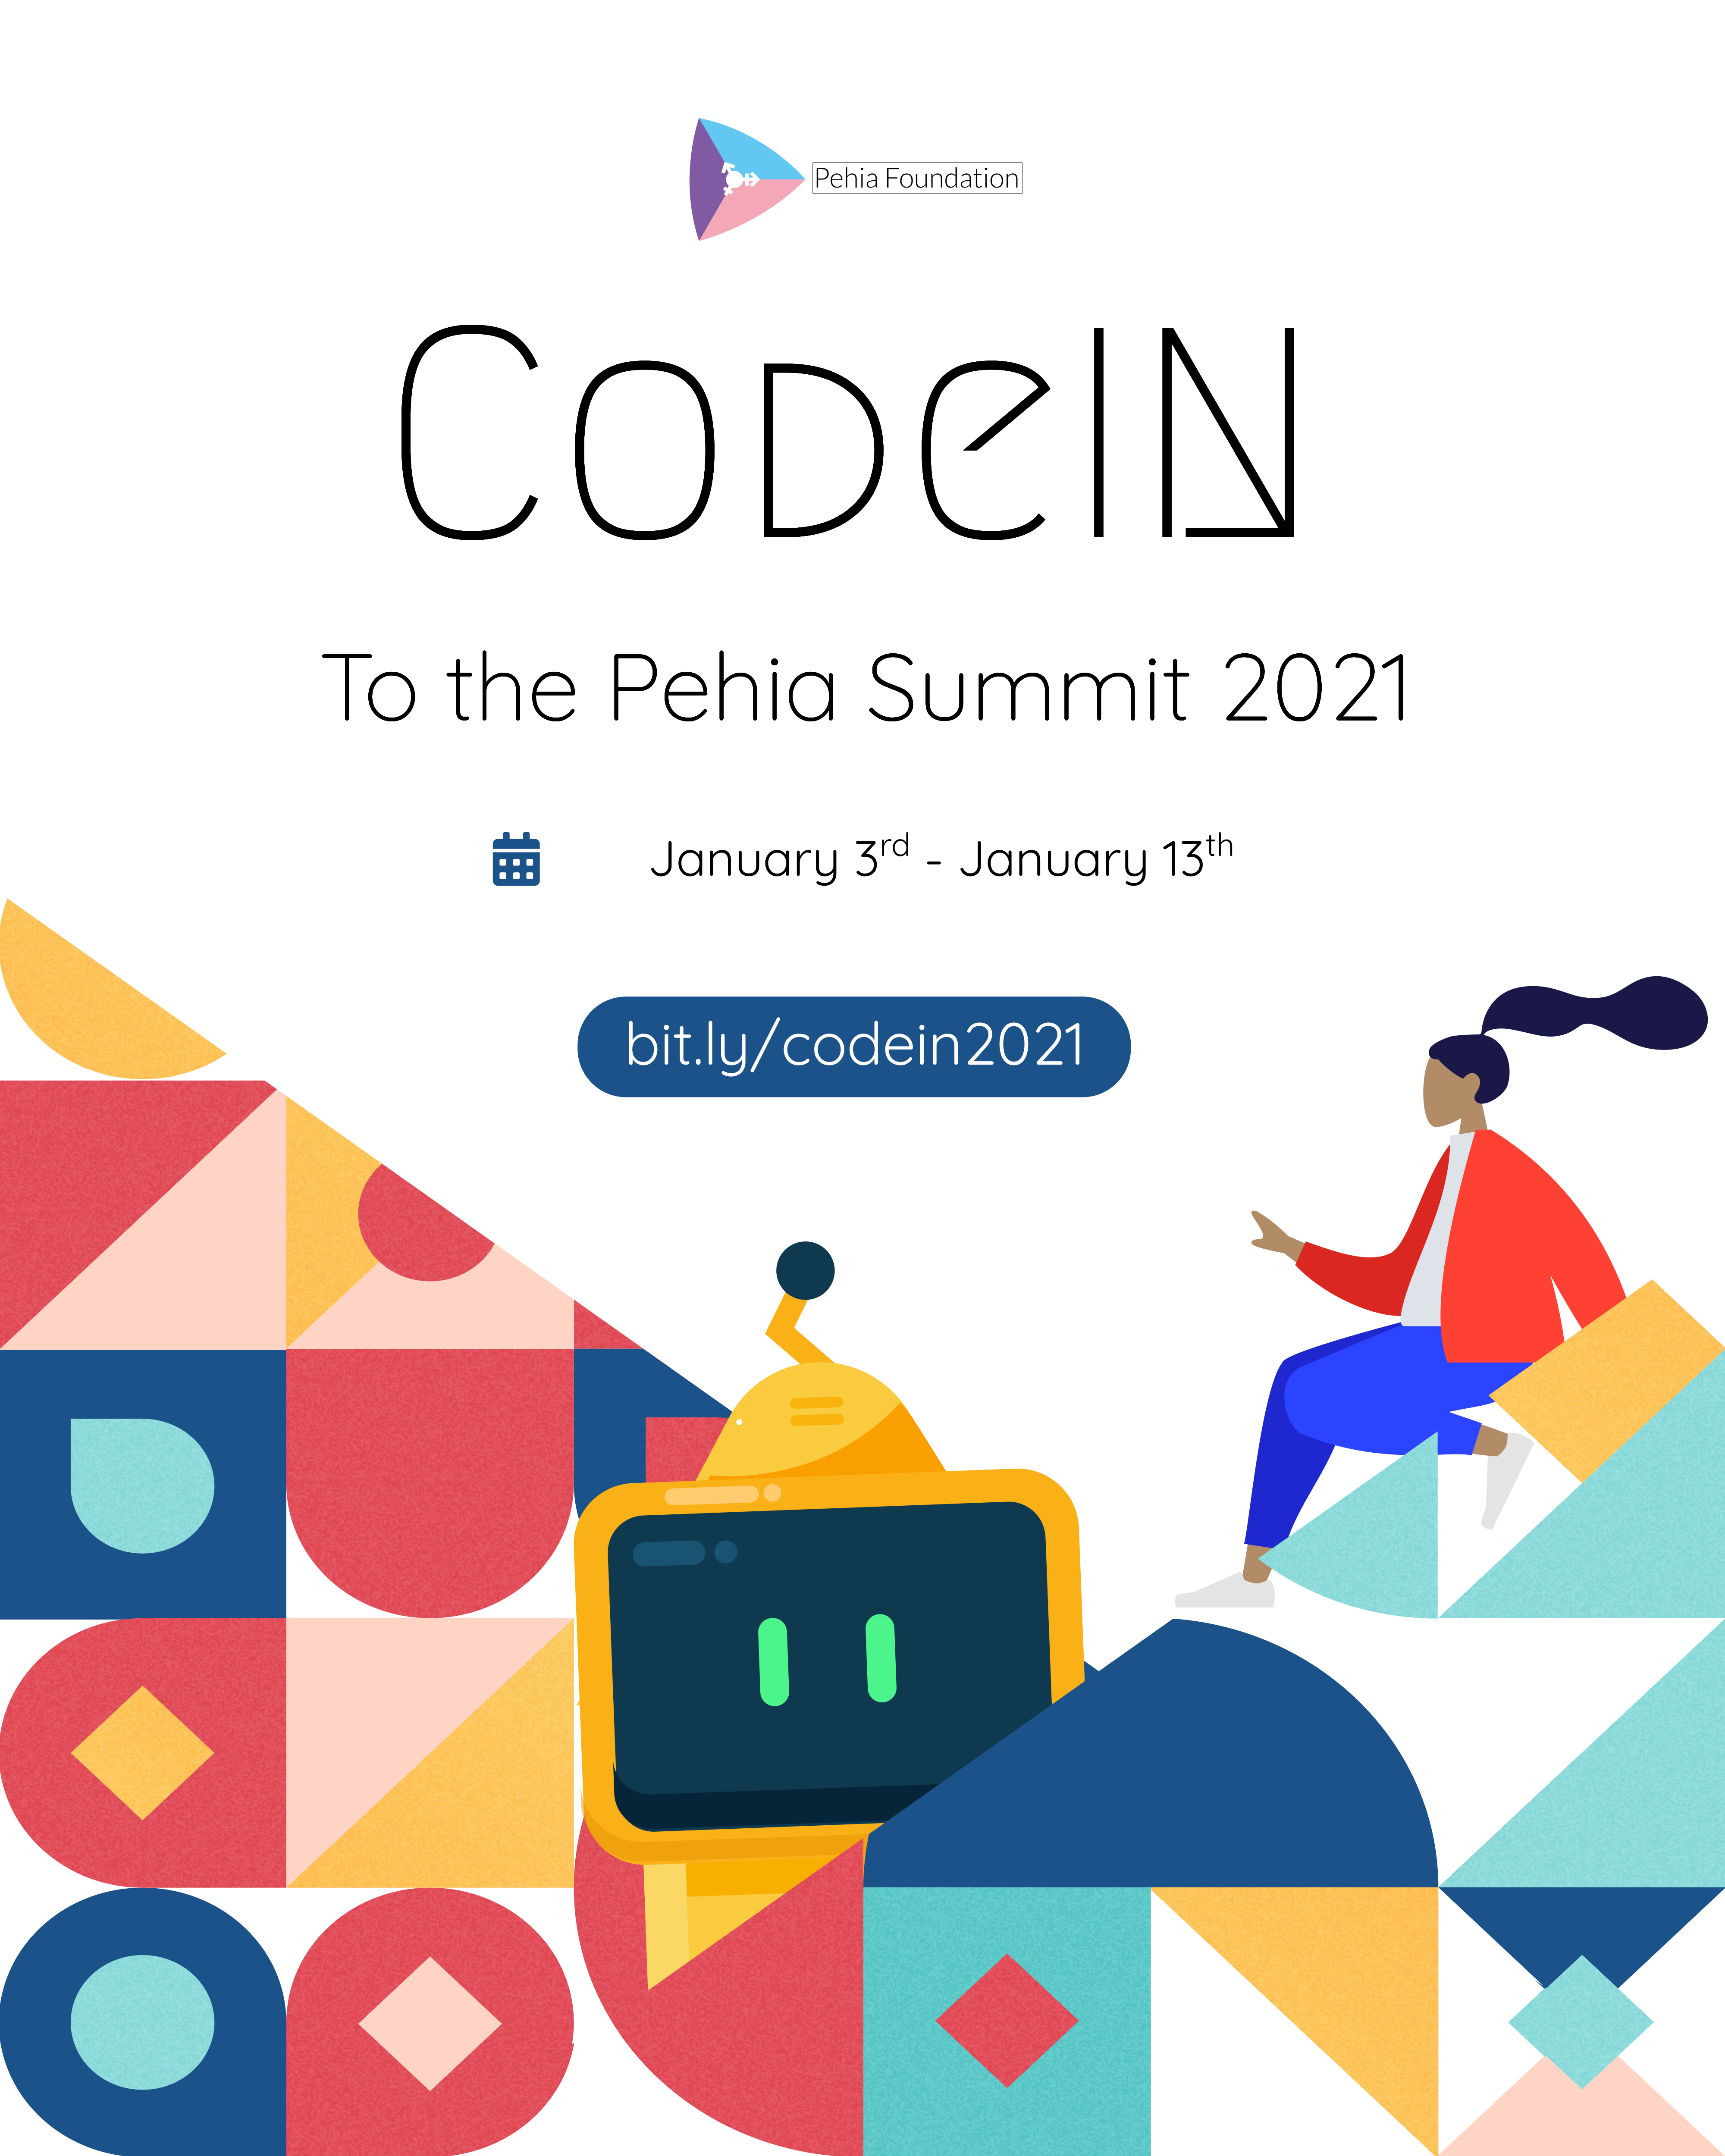
\includegraphics[width=.9\linewidth]{././codein.png}
\caption{CodeIn, Pehia Summit (2021)}
\end{figure}
\end{column}
\begin{column}{0.25\columnwidth}
\begin{figure}[htbp]
\centering

\includegraphics[width=.9\linewidth]{././cpfdraft.png}
\caption{CPF, MiniDebConf India (2021)}
\end{figure}
\end{column}
\end{columns}
\end{frame}
\section*{FOSS Design Tools}
\label{sec:org7ad5e41}
\begin{frame}[label={sec:org51e1cb3}]{Inkscape}
\begin{columns}
\begin{column}{0.5\columnwidth}
\begin{itemize}
\item Vector Graphics tool
\item Uses SVG as base format
\item Flexible
\item Advanced features (Object Transformations, Bitmap tracing and more!)
\end{itemize}
\end{column}
\begin{column}{0.5\columnwidth}
\begin{figure}[htbp]
\centering
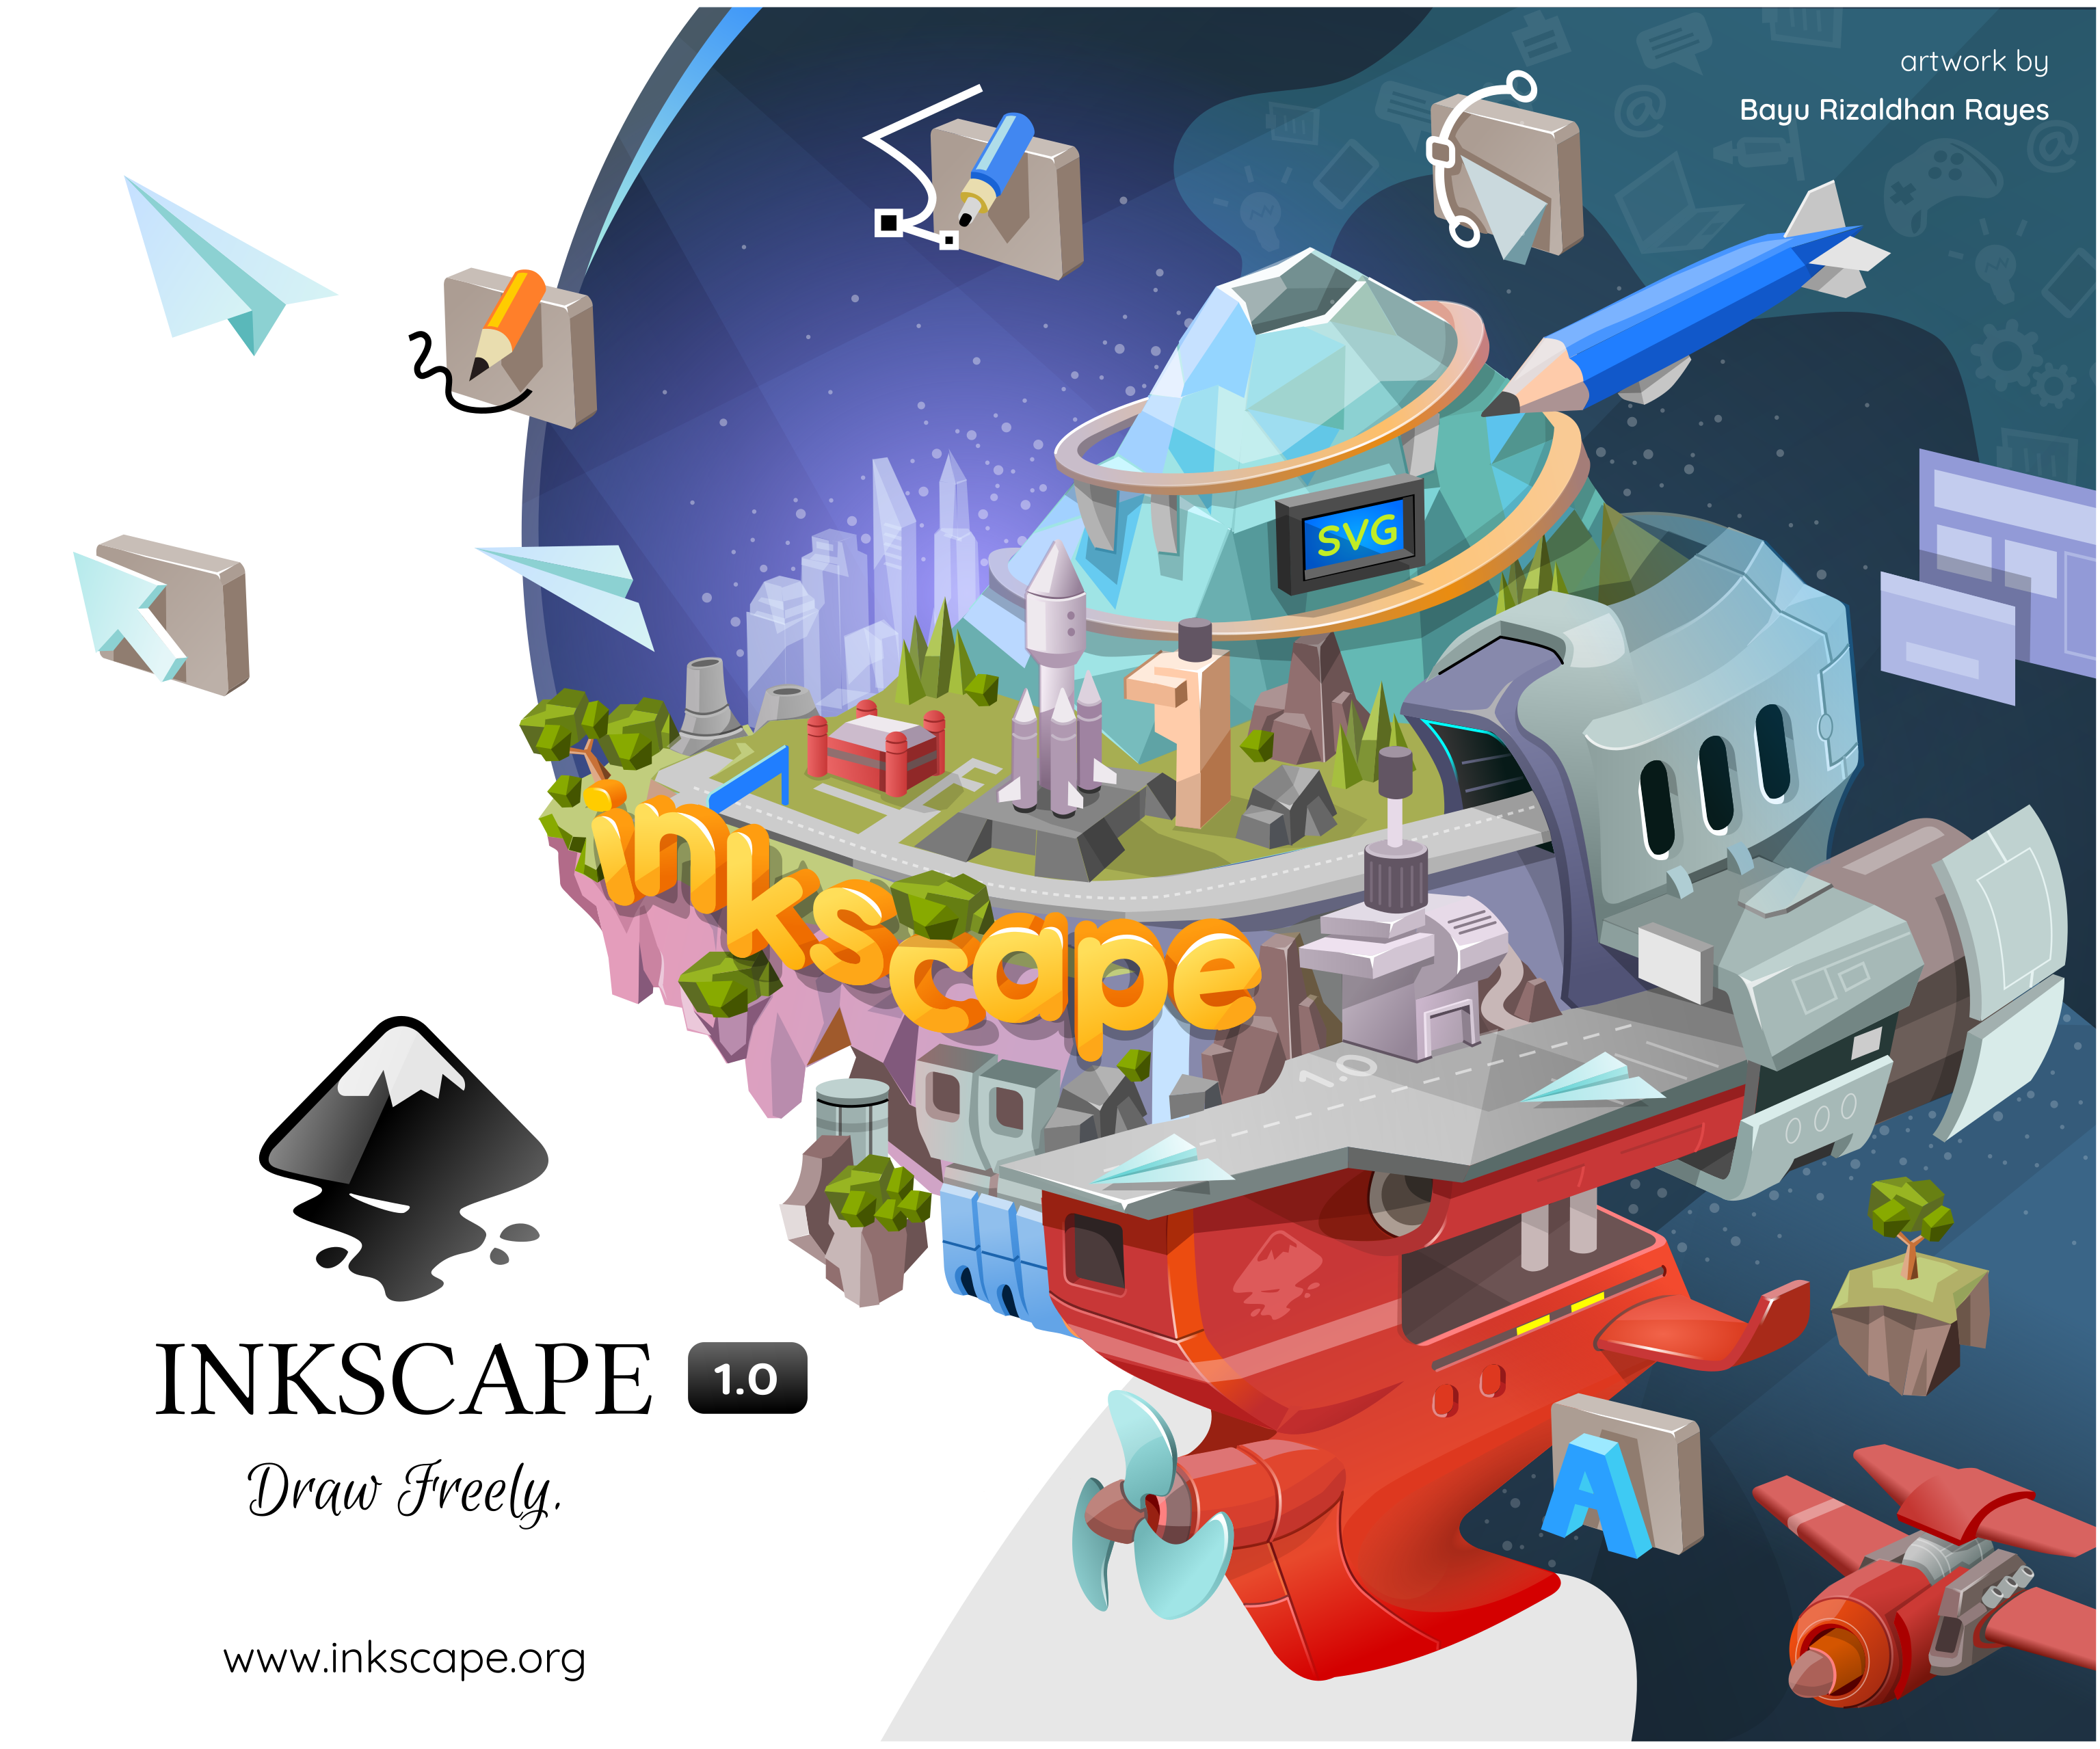
\includegraphics[width=.9\linewidth]{././inkscape.png}
\caption{Designed Using Inkscape}
\end{figure}
\end{column}
\end{columns}
\end{frame}
\begin{frame}[label={sec:org1187a2d}]{Gimp}
\begin{columns}
\begin{column}{0.5\columnwidth}
\begin{itemize}
\item \alert{G} NU  \alert{I} mage  \alert{M} anipulation  \alert{P} rogram
\item 25 years and still going strong.
\item photo retouching program, an online batch processing system, a mass production image renderer, an image format converter and more.
\end{itemize}
\end{column}
\begin{column}{0.5\columnwidth}
\begin{figure}[htbp]
\centering
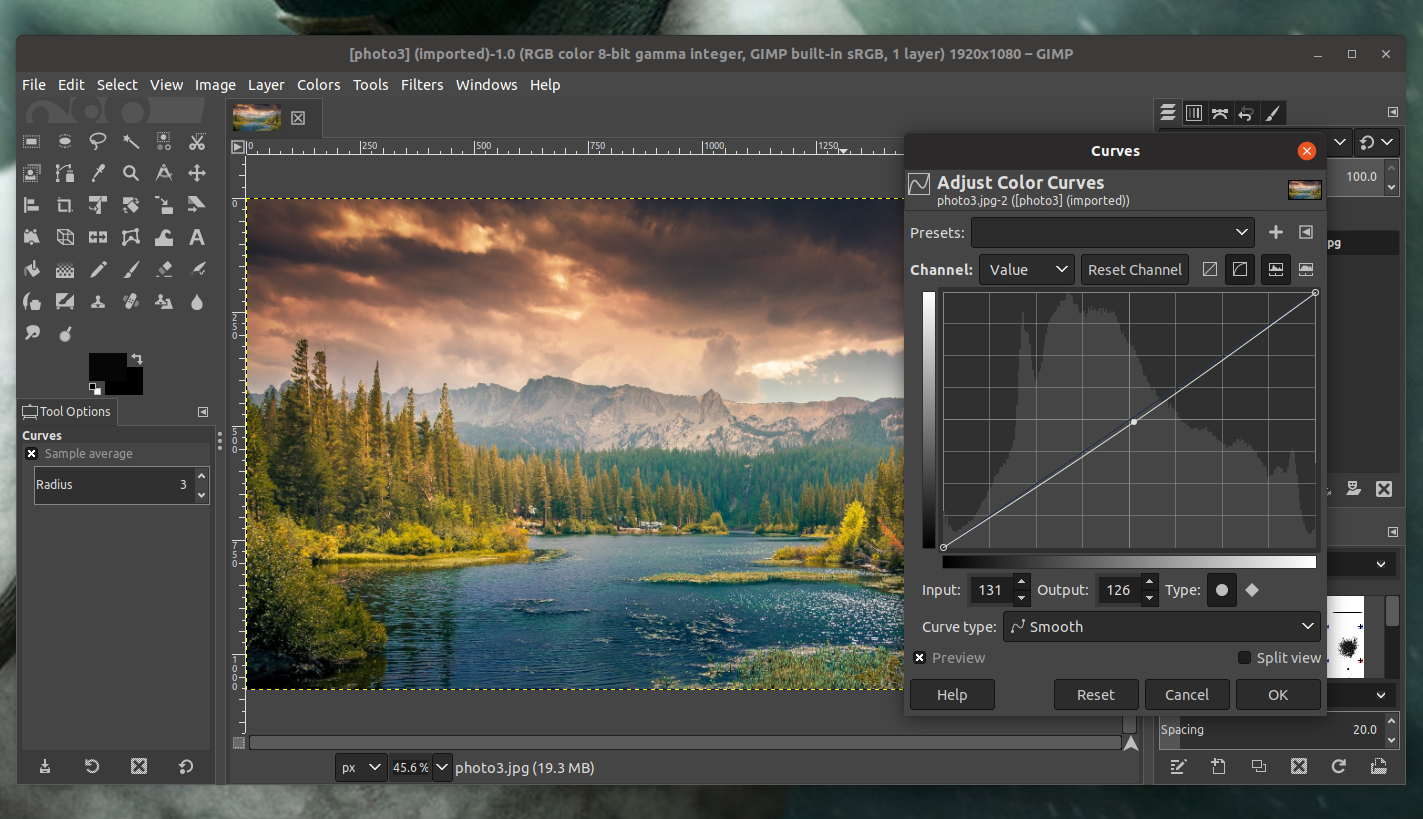
\includegraphics[width=.9\linewidth]{././gimp.png}
\caption{Gimp in Action}
\end{figure}
\end{column}
\end{columns}
\end{frame}
\begin{frame}[label={sec:org0699d60}]{Krita}
\begin{columns}
\begin{column}{0.4\columnwidth}
\begin{itemize}
\item Professional FREE and open source painting program.
\item Made by artists that want to see affordable art tools for everyone.
\item Beautiful Brushes, Animation, HDR, Scripting and more!
\end{itemize}
\end{column}
\begin{column}{0.6\columnwidth}
\begin{figure}[htbp]
\centering
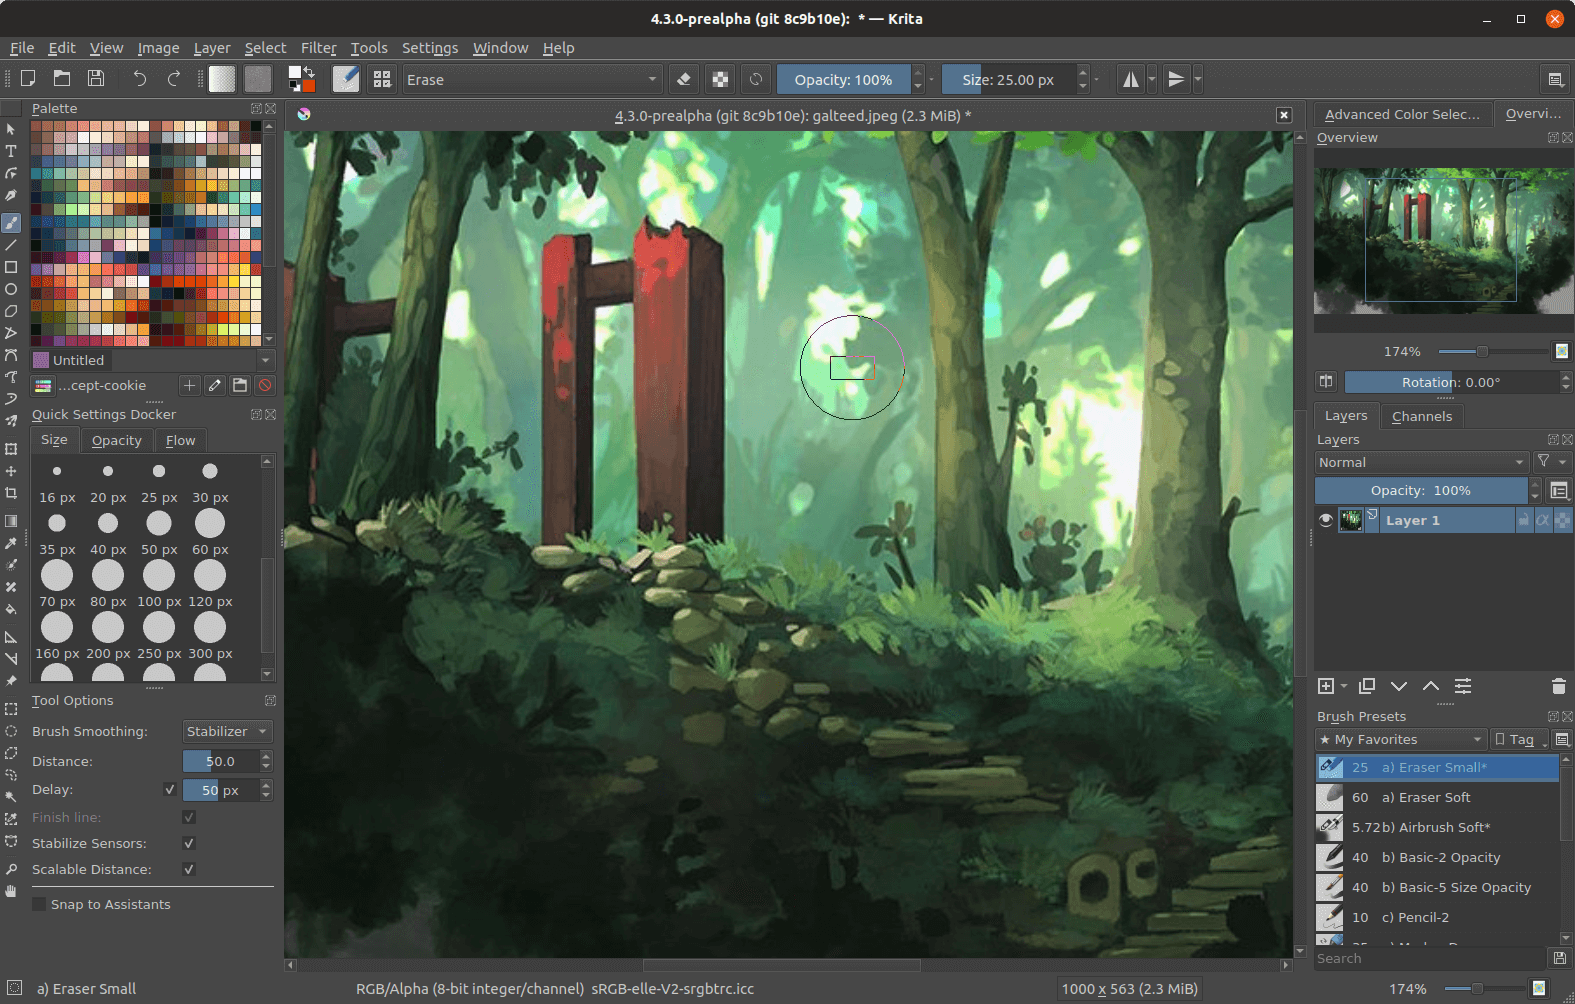
\includegraphics[width=.9\linewidth]{./krita.png}
\caption{Krita in Action}
\end{figure}
\end{column}
\end{columns}
\end{frame}
\begin{frame}[label={sec:org48bd4b3}]{Pencil}
\begin{columns}
\begin{column}{0.4\columnwidth}
\begin{itemize}
\item The best UI/UX Open Source tool out there.
\item Slow Development.
\item Prototyping, GUI mockup, export to web page etc.
\end{itemize}
\end{column}
\begin{column}{0.6\columnwidth}
\begin{figure}[htbp]
\centering
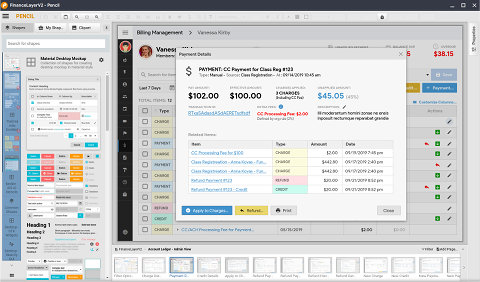
\includegraphics[width=.9\linewidth]{./pencil.png}
\caption{Pencil in Action}
\end{figure}
\end{column}
\end{columns}
\end{frame}
\section*{Thanks}
\label{sec:org0be0415}
\begin{frame}[label={sec:org6d27a22}]{Thanks for Listening}
\begin{columns}
\begin{column}{0.6\columnwidth}
\begin{itemize}
\item If I can do it so can you.
\item Popularize and normalize FOSS tools for Art.
\item Tools made with \alert{\alert{<3}} Rock!
\end{itemize}
\end{column}
\end{columns}
\end{frame}
\end{document}
